\section{The Copenhagen Interpretation and the EPR-Bohm Paradox\label{eprsec}}
Given the equations (\ref{spintrans1}) and (\ref{spintrans2}) that  relate the states $\ket*{\uvbpm{a}}$ and $\ket*{\uvbpm{b}}$ to each other, we can calculate probabilities such as the probability a particle will be measured to be in the $\ket*{\uvbp{a}}$-state given that it is in the $\ket*{\uvbp{b}}$-state. There however arises the question of what the physical meaning of one of these states is. Clearly, the $\ket*{\uvbp{b}}$-state says something about the spin of a particle; but is this a complete description of the particle's spin state? For the $\ket*{\uvbp{b}}$-state only tells us what the outcome of a spin measurement would be along one particular axis $\uvb{b}$. For a spin measurement along another axis $\uvb{a}\neq\pm\uvb{b}$, $\ket*{\uvbp{b}}$ only tells us the probabilities (via equation (\ref{spintrans1}) and the Born Rule) that the measurement outcome would be $\ket*{\uvbp{a}}$ or $\ket*{\uvbm{a}}$ -- but the $\ket*{\uvbp{b}}$-state doesn't determine either of these outcomes. So we want to know whether this indetermination of the measurement outcome along the $\uvb{a}$-axis is merely a reflection of our lack of knowledge of a more complete specification of the particle's spin state, or alternatively, whether the  $\ket*{\uvbp{b}}$-state is a complete description of the spin state of the particle so that there is no fact of the matter about what spin state the particle would be found to be in along the $\uvb{a}$-axis until a measurement of spin along the $\uvb{a}$-axis is made. 

Now Bohr and Heisenberg believed the latter to be the case. This was because their mathematical formalism of quantum physics implied that there are physical quantities of particles that couldn't be simultaneously determined. For example, their mathematical formalism is incapable of representing a particle which has a definite spin in both the $\uvb{a}$-direction and the $\uvb{b}$-direction when $\uvb{a}\neq\pm\uvb{b}.$ So when a particle that is in the $\ket*{\uvbp{b}}$-state is measured along the $\uvb{a}$-axis and is found to be in the $\ket*{\uvbp{a}}$-state, there is a so-called collapse of the $\ket*{\uvbp{b}}$-state:
$$ \ket*{\uvbp{b}}= \cos(\theta/2)\ket*{\uvbp{a}}+\sin(\theta/2) \ket*{\uvbm{a}}\xrightarrow{\text{Collapse!!}}\ket*{\uvbp{a}}$$
so that after the measurement, the particle is no longer in the $\ket*{\uvbp{b}}$-state. This interpretation of the quantum state as a complete physical description in which the state collapses to another state upon measurement is known as the \textbf{Copenhagen Interpretation}\index{Copenhagen Interpretation}.

Einstein, Podolsky, and Rosen, however, strongly objected to the Copenhagen Interpretation, and they introduced their EPR paradox to explain what troubled them.\footnote{See \cite{EinsteinPodolskyRosen}.} The EPR paradox was originally expressed in terms of the position and momentum of a particle, but it was Bohm who translated the EPR paradox to the context of spin,\footnote{e.g. see \cite[p. 29, Ch. 5 sec. 3, and Ch. 22 sec. 19]{BohmQuantumTheory}. } and this is the version we will consider here.   

The EPR-Bohm paradox arises in the context of particle pairs known as spin singlets. A \textbf{spin singlet}\index{spin singlet} describes the state of two particles which a single particle of zero spin has decayed into. For example, a high energy \textbf{photon}\index{photon}, that is, a particle of light, can decay into a negatively charged electron, and a positively charged positron (where a \textbf{positron}\index{positron} is a fundamental particle like an electron but of opposite charge). Since spin is a conserved physical quantity, the spin of the two particles $q_A$ and $q_B$ of a spin singlet state must be equal and opposite when measured along the same axis, no matter what direction this axis happens to point in. The existence of spin singlet states thus raises the question of what the physical mechanism or principle is that ensures two experimenters, Alice and Bob say, will always obtain opposite spin measurement results if Alice measures the spin of particle $q_A$, and Bob measures the spin of particle $q_B$ along the same axis. There is of course no experiment that could prove that Alice and Bob will always obtain opposite spin measurements, and there are some interpretations of quantum physics such as the GRW spontaneous collapse theory\footnote{See \cite{sep-qm-collapse}.} which predict that very occasionally Alice and Bob would obtain the same spin measurement result. But in this dissertation, we will assume that all measurements are consistent with \textbf{standard quantum theory}\index{standard quantum theory}. In other words, we assume that the physical world can be described by quantum states\footnote{In standard quantum theory, we remain agnostic as to whether a quantum state provides a complete description of the physical world, or whether it needs to be supplemented by some additional information in order to obtain a complete description.} that evolve over time according to the Schr\"{o}dinger equation, and that the probability of a system being found to be in one state given that it is in another state will be given by the Born Rule.  In particular, under the assumption of standard quantum theory, it will follow that Alice and Bob will always obtain opposite spin results when performing measurements along the same axis of two particles in the spin singlet state. 

Now naively, one would expect that if the spin of $q_A$ were to be measured, then this would have no effect on any spin-measurement of $q_B$. This assumption is a special case of \textbf{Einstein's locality principle}\index{Einstein's locality principle}:\label{EinsteinLocalityPrinciple} For two spatially separated systems $S_1$ and $S_2$,  the real factual situation of the system $S_2$ should be independent of what is done to the system $S_1$.\footnote{Einstein expressed this locality principle in his autobiographical notes: ``But on one supposition we should, in my opinion, absolutely hold fast: the real factual situation of the system $S_2$ is independent of what is done with the system $S_1$, which is spatially separated from the former.'' \cite[p. 85]{EinsteinLocality}.} If Einstein's locality principle holds, we would be able to attribute a state $\ket{\alpha}_A$ to particle $q_A$, and a state $\ket{\beta}_B$ to particle $q_B$, so that if Alice were to perform a Stern-Gerlach experiment on particle $q_A$ in which one of the possible outcomes was a spin state $\ket*{\alpha'}_A$, then by the Born Rule, the probability Alice would find $q_A$ to be in state $\ket{\alpha'}_A$ would be $|\ip{\alpha'}{\alpha}_A|^2$. Likewise, if Bob were to perform a Stern-Gerlach experiment on particle $q_B$ in which one of the possible outcomes was a spin state $\ket*{\beta'}$, then the probability Bob would find $q_B$ to be in state $\ket{\beta'}_B$ would be $|\ip{\beta'}{\beta}_B|^2$. 

Now in order to decide how to represent the joint state of the particles $q_A$ and $q_B$, we recall that  in probability theory, we say that two events $X$ and $Y$ are \textbf{statistically independent}\index{statistical independence} if and only if 
\begin{equation}\label{indep}
    P(X,Y)=P(X)P(Y)
\end{equation}
where $P(X)$ is the probability that $X$ occurs, $P(Y)$ is the probability that $Y$ occurs, and $P(X,Y)$ is the probability that both $X$ and $Y$ both occur. We define the \textbf{conditional probability}\index{conditional probability} $P(X|Y)$ of $X$ given $Y$ to be
\begin{equation}\label{conditionaprob}
P(X|Y)= \frac{P(X,Y)}{P(Y)}.
\end{equation}
From (\ref{indep}), it is easy to see that when $X$ and $Y$ are independent, $P(X|Y)=P(X)$. We also say that two events $X$ and $Y$ are \textbf{conditionally independent}\index{conditional independence} given some third event $Z$ if and only if 
\begin{equation}\label{indepcond}
P(X,Y|Z)=P(X|Z)P(Y|Z)
\end{equation} where $P(X|Z)$ is the conditional probability that $X$ occurs given $Z$, $P(Y|Z)$ is the conditional probability that $Y$ occurs given $Z$, and $P(X,Y|Z)$ is the conditional probability that both $X$ and $Y$  occur given $Z$.   

Now if $q_A$ can be described by the $\ket*{\alpha}_A$-state and $q_B$ can be described by the $\ket*{\beta}_B$-state, the Born Rule implies that the conditional probability that Alice would measure her particle to be in the state $\ket*{\alpha'}_A$ is not going to depend on $\ket*{\beta}_B$,  and so  $P(\alpha'|\alpha,\beta)=P(\alpha'|\alpha)$. Likewise, $P(\beta'|\alpha,\beta)=P(\beta'|\beta)$. 
Therefore, if Alice and Bob's measurement outcomes are conditionally independent, then according to (\ref{indepcond}) and the Born Rule, we would obtain the conditional probability
\begin{equation}\label{indepprob}
    P_{AB}(\alpha',\beta'|\alpha,\beta)=|\ip{\alpha'}{\alpha}_A|^2\times|\ip{\beta'}{\beta}_B|^2=|\ip{\alpha'}{\alpha}_A\ip{\beta'}{\beta}_B|^2.
\end{equation}
This suggests that if we write $\ket{\alpha}_A\ket{\beta}_B$ for the state of the composite system of both particles, then the bra-ket of $\ket{\alpha'}_A\ket{\beta'}_B$ and $\ket{\alpha}_A\ket{\beta}_B$ 
would be
\begin{equation}\label{innerprod}
    \prescript{}{B}{ \bra*{\beta'}}\prescript{}{A}{\ip*{\alpha'}{\alpha}}_A\ket*{\beta}_B=\ip{\alpha'}{\alpha}_A\ip{\beta'}{\beta}_B,
\end{equation}
and we extend this bracket to sums of states so that it satisfies the linearity property (see page \pageref{linearity}).
However, when the particles $q_A$ and $q_B$ form a spin singlet, it will not be possible to express their joint state as $\ket{\alpha}_A\ket{\beta}_B$ because otherwise, according to (\ref{indepprob}), we will always be able to find a direction $\uvb{a}$ such that $P_{AB}(\uvbp{a},\uvbp{a}|\alpha,\beta)\neq 0$, whereas in reality, the state $Z$ describing the singlet has to satisfy $P_{AB}(\uvbp{a},\uvbp{a}|Z)=0$ for all  $\uvb{a}$.
But it turns out that the summation of states:
\begin{equation}\label{bell}
    \ket*{\Psi_{\text{Bell}}}=\frac{1}{\sqrt{2}}(\ket*{\uvbp{a}}_A\ket*{\uvbm{a}}_B-\ket*{\uvbm{a}}_A\ket*{\uvbp{a}}_B).
\end{equation}
can describe the singlet state of the two particles. We refer to the state (\ref{bell}) as a \textbf{Bell state}\index{Bell state}.\footnote{By convention, the states $ \frac{1}{\sqrt{2}}(\ket*{\uvbp{a}}_A\ket*{\uvbm{a}}_B+\ket*{\uvbm{a}}_A\ket*{\uvbp{a}}_B)$, $ \frac{1}{\sqrt{2}}(\ket*{\uvbp{a}}_A\ket*{\uvbp{a}}_B-\ket*{\uvbm{a}}_A\ket*{\uvbm{a}}_B)$, and $ \frac{1}{\sqrt{2}}(\ket*{\uvbp{a}}_A\ket*{\uvbp{a}}_B+\ket*{\uvbm{a}}_A\ket*{\uvbm{a}}_B)$ are also referred to as Bell states.} If the composite system is in the Bell state $\ket*{\Psi_{\text{Bell}}}$, then according to the Born Rule, the probability that Alice measures her particle to be in state $\ket*{\alpha}$ and Bob measures his particle to be in the state $\ket*{\beta}$ will be:
\begin{equation}
\begin{split}
    P_{AB}(\alpha,\beta|\Psi_{\text{Bell}})&=|\prescript{}{B}{ \bra*{\beta}}\prescript{}{A}{ \ip{\alpha}{\Psi_{\text{Bell}}}}|^2\\
        &=\frac{1}{2}|\ip*{\alpha}{\uvbp{a}}_A\ip*{\beta}{\uvbm{a}}_B-\ip*{\alpha}{\uvbm{a}}_A\ip*{\beta}{\uvbp{a}}_B|^2
\end{split}
\end{equation}
This means that whatever axis Bob decides to measure along, if Alice measures her particle along the $\uvb{a}$-axis, then the Born Rule predicts that she will measure the particle to be in either the $\ket*{\uvbp{a}}_A$-state or the $\ket*{\uvbm{a}}_A$-state, each with probability of $\frac{1}{2}$.\footnote{To see this, suppose Bob performs his measurement along an arbitrary axis $\uvb{b}$. Then the probability Alice measures her particle to be in the $\ket*{\uvbp{a}}$-state will be 
\begin{equation}
    \begin{split}
        P_{AB}(\uvbp{a},\uvbp{b}|\Psi_{\text{Bell}})&+P_{AB}(\uvbp{a},\uvbm{b}|\Psi_{\text{Bell}})= \\
        =&\frac{1}{2}\big| \ip*{\uvbp{a}}{\uvbp{a}}_A\ip*{\uvbp{b}}{\uvbm{a}}_B-\ip*{\uvbp{a}}{\uvbm{a}}_A\ip*{\uvbp{b}}{\uvbp{a}}_B\big|^2\\
        &+\frac{1}{2}\big|\ip*{\uvbp{a}}{\uvbp{a}}_A\ip*{\uvbm{b}}{\uvbm{a}}_B-\ip*{\uvbp{a}}{\uvbm{a}}_A\ip*{\uvbm{b}}{\uvbp{a}}_B\big|^2\\
        =&\frac{1}{2}\big|\ip*{\uvbp{b}}{\uvbm{a}}_B|^2+\frac{1}{2}|\ip*{\uvbm{b}}{\uvbm{a}}_B\big|^2=\frac{1}{2}
    \end{split}
\end{equation} 
where on the last line we have used the fact that 
$$\ket*{\uvbm{a}}_B=\ket*{\uvbp{b}}_B\ip*{\uvbp{b}}{\uvbm{a}}_B+\ket*{\uvbm{b}}\ip*{\uvbm{b}}{\uvbm{a}}_B$$
and 
$$\ip*{\uvbm{a}}{\uvbm{a}}_B=1,\quad\ip*{\uvbpm{b}}{\uvbpm{b}}_B=1,\quad\text{and}\quad \ip*{\uvbpm{b}}{\uvbmp{b}}_B=0$$
so that 
$$|\ip*{\uvbp{b}}{\uvbm{a}}_B|^2+\ip*{\uvbm{b}}{\uvbm{a}}_B|^2=1.$$
} But also, the Born Rule implies that if both Alice and Bob measure their respective particles along the same $\uvb{a}$-axis, then the probability Bob will measure his particle to have the same spin as Alice's particle will be zero, and the probability that Bob measures his particle to have the opposite spin from Alice's particle will be one.\footnote{This is because the probability Alice and Bob will measure their particles to have the same spin will be 
\begin{equation*}
\begin{split}
    P_{AB}(\uvbp{a},\uvbp{a}|\Psi_{\text{Bell}})&+P_{AB}(\uvbm{a},\uvbm{a}|\Psi_{\text{Bell}})= \\
    =&\frac{1}{2}\big| \ip*{\uvbp{a}}{\uvbp{a}}_A\ip*{\uvbp{a}}{\uvbm{a}}_B-\ip*{\uvbp{a}}{\uvbm{a}}_A\ip*{\uvbp{a}}{\uvbp{a}}_B\big|^2\\
    &+\frac{1}{2}\big|\ip*{\uvbm{a}}{\uvbp{a}}_A\ip*{\uvbm{a}}{\uvbm{a}}_B-\ip*{\uvbm{a}}{\uvbm{a}}_A\ip*{\uvbm{a}}{\uvbp{a}}_B\big|^2=0,
\end{split}
\end{equation*}
and the probability Alice and Bob will measure their particles to have different spins will be
\begin{equation*}
\begin{split}
    P_{AB}(\uvbp{a},\uvbm{a}|\Psi_{\text{Bell}})&+P_{AB}(\uvbm{a},\uvbp{a}|\Psi_{\text{Bell}})= \\
    =&\frac{1}{2}\big| \ip*{\uvbp{a}}{\uvbp{a}}_A\ip*{\uvbm{a}}{\uvbm{a}}_B-\ip*{\uvbp{a}}{\uvbm{a}}_A\ip*{\uvbm{a}}{\uvbp{a}}_B\big|^2\\
    &+\frac{1}{2}\big|\ip*{\uvbm{a}}{\uvbp{a}}_A\ip*{\uvbp{a}}{\uvbm{a}}_B-\ip*{\uvbm{a}}{\uvbm{a}}_A\ip*{\uvbp{a}}{\uvbp{a}}_B\big|^2=1.
\end{split}
\end{equation*}} 
These probabilities predicted by the Born Rule using the Bell state $\ket*{\Psi_{\text{Bell}}}$ correspond to the probabilities observed experimentally. Also note that despite the of appearance the formula (\ref{bell}), $\ket*{\Psi_{\text{Bell}}}$ is independent of the axis $\uvb{a}$. That is, for any other direction $\uvb{b}$, it can be shown that,
\begin{equation}\label{bellstate2}\frac{1}{\sqrt{2}}(\ket*{\uvbp{a}}_A\ket*{\uvbm{a}}_B-\ket*{\uvbm{a}}_A\ket*{\uvbp{a}}_B)=\frac{1}{\sqrt{2}}(\ket*{\uvbp{b}}_A\ket*{\uvbm{b}}_B-\ket*{\uvbm{b}}_A\ket*{\uvbp{b}}_B).\protect\footnotemark\end{equation}
\footnotetext{\label{bellstate2pf}To see this, using the transformation rules given in equation (\ref{spintrans}) we have 
\begin{align*}\frac{1}{\sqrt{2}}(\ket*{\uvbp{b}}\ket*{\uvbm{b}}&-\ket*{\uvbm{b}}\ket*{\uvbp{b}})\\
      &=\frac{1}{\sqrt{2}}((\cos(\theta/2)\ket*{\uvbp{a}}+\sin(\theta/2)\ket*{\uvbm{a}})(\cos(\theta/2)\ket*{\uvbm{a}}-\sin(\theta/2)\ket*{\uvbp{a}})\\
&\quad-(\cos(\theta/2)\ket*{\uvbm{a}}-\sin(\theta/2)\ket*{\uvbp{a}})(\cos(\theta/2)\ket*{\uvbp{a}}+\sin(\theta/2)\ket*{\uvbm{a}}))\\ 
&=\frac{1}{\sqrt{2}}(\cos(\theta/2)\ket*{\uvbp{a}}\cos(\theta/2)\ket*{\uvbm{a}}-\cos(\theta/2)\ket*{\uvbp{a}}\sin(\theta/2)\ket*{\uvbp{a}}\\
&\quad+\sin(\theta/2)\ket*{\uvbm{a}}\cos(\theta/2)\ket*{\uvbm{a}}-\sin(\theta/2)\ket*{\uvbm{a}}\sin(\theta/2)\ket*{\uvbp{a}}\\
&\quad-\cos(\theta/2)\ket*{\uvbm{a}}\cos(\theta/2)\ket*{\uvbp{a}}-\cos(\theta/2)\ket*{\uvbm{a}}\sin(\theta/2)\ket*{\uvbm{a}}\\
&\quad+\sin(\theta/2)\ket*{\uvbp{a}}\cos(\theta/2)\ket*{\uvbp{a}}+
\sin(\theta/2)\ket*{\uvbp{a}}\sin(\theta/2)\ket*{\uvbm{a}})\\
&=\frac{1}{\sqrt{2}}((\cos[2](\theta/2)+\sin[2](\theta/2))\ket*{\uvbp{a}}\ket*{\uvbm{a}}-(\cos[2](\theta/2)+\sin[2](\theta/2))\ket*{\uvbm{a}}\ket*{\uvbp{a}})\\
&=\frac{1}{\sqrt{2}}(\ket*{\uvbp{a}}\ket*{\uvbm{a}}-\ket*{\uvbm{a}}\ket*{\uvbp{a}}).
\end{align*}}
Therefore, if Alice had chosen to measure her particle along the $\uvb{b}$-axis rather than the $\uvb{a}$-axis, she would still obtain equal probabilities for finding her particle to be in either the state $\ket*{\uvbp{b}}_A$ or $\ket*{\uvbm{b}}_A$, and the same equal probabilities for Bob's measurement outcomes hold as well.

Now although attributing the state $\ket*{\Psi_{\text{Bell}}}$ successfully determines the experimentally observed probabilities for  Alice and Bob's spin measurement outcomes, this fact spells trouble for the Copenhagen interpretation. For if we stipulate that $\ket*{\Psi_{\text{Bell}}}$ is a complete description of the spin state of the spin-singlet, then assuming Alice makes her measurement first and obtains the measurement outcome $\ket*{\uvbp{a}}_A$, then as this measurement outcome is established there will be a collapse of the state 
$$\ket*{\Psi_{\text{Bell}}}=\frac{1}{\sqrt{2}}(\ket*{\uvbp{a}}_A\ket*{\uvbm{a}}_B-\ket*{\uvbm{a}}_A\ket*{\uvbp{a}}_B)\xrightarrow{\text{Collapse!!}}\ket*{\uvbp{a}}_A\ket*{\uvbm{a}}_B$$
Thus, according to the Copenhagen interpretation, prior to Alice's measurement, the real factual situation of particle $q_B$ will be indeterminate, but once Alice has made her measurement and obtained the outcome $\ket*{\uvbp{a}}_A$, the real factual situation of particle $q_B$ will be expressed by the determinate state $\ket*{\uvbm{a}}_B$. Thus, in the state collapse that Alice brings about via her measurement, there is a violation of Einstein's locality principle. 

But things get even worse when we take Einstein's theory of special relativity into consideration. For according to Einstein's theory of relativity, the order in which Alice and Bob perform their measurements is going to depend on which inertial frame of reference one is in.\footnote{In special relativity, an inertial frame of reference is a spacetime coordinate system $(t, x, y, z)$ in which all objects which have no forces acting on them have trajectories that are straight lines. Thus, we can move to another inertial frame by moving to a reference frame with constant velocity $\vb{v}$ with respect to the first reference frame. In the case when $\vb{v}=(v, 0, 0)$, Einstein's theory of special relativity tells us that under such a “boost”, spacetime coordinates will transform as $(t,\vb{x})\rightarrow(t',x',y',z')=(\gamma\big(t - \frac{vx}{c^2}\big),\gamma(x-vt),y,z)$ where $c$ is the speed of light and $\gamma=\Big(\sqrt{1-\frac{v^2}{c^2}}\Big)^{-1}.$ } Thus, if we are moving at one velocity, it may appear that Alice makes her measurement first meaning that Alice causes the state collapse and thus affects the state of Bob's particle, whereas if we are moving at another velocity, it may appear that Bob makes his measurement first causing the state to collapse and thus affects the state of Alice's particle. Once the collapse has occurred, there is no further collapse when the second experimenter makes his or her measurement along the same axis as the first experimenter. Thus, the thesis of the Copenhagen interpretation that it is the act of measurement that causes the state to collapse is not compatible with Einstein's theory of special relativity, for if special relativity is correct, then one and the same measurement both will and will not cause the state to collapse depending upon which frame of reference one is in.

Therefore, if one is more convinced (as most physicists are) of the truth of Einstein's theory of relativity than the truth of the Copenhagen interpretation, then one must reject the Copenhagen interpretation. Thus, in the light of the EPR-Bohm paradox we need an alternative to the Copenhagen interpretation of quantum states that can account for how the two experimenters of the paradox always obtain opposite results when they make their measurement along the same axis. The obvious approach to take is to suppose that the quantum state $\ket*{\Psi_{\text{Bell}}}$ is an incomplete description of the spin state of the two particles. This is the hidden variables approach, but as we will see shortly, this approach is also problematic. But before we consider the hidden variables approach, we will turn to what is traditionally considered to be one of the most troubling aspect of the Copenhagen interpretation, namely the possibility of scenarios exemplified by Schr\"{o}dinger's cat thought experiment.

\section{Schr\"{o}dinger's Cat\protect\footnotemark}\footnotetext{For Schr\"{o}dinger's original reference to his thought experiment, see \cite{SchrondingerOrig}. For an English translation, see \cite{SchrondingerEnglish}.}
*********************************

-- for instance, in a Schr\"{o}dinger cat-like experiment, there would be a stress-energy tensor distribution corresponding to both the cat being alive and the cat being dead in the same world as depicted in figure \ref{deadlivecat}.
\begin{figure}[ht!]
  \captionsetup{justification=justified}
  \centering
  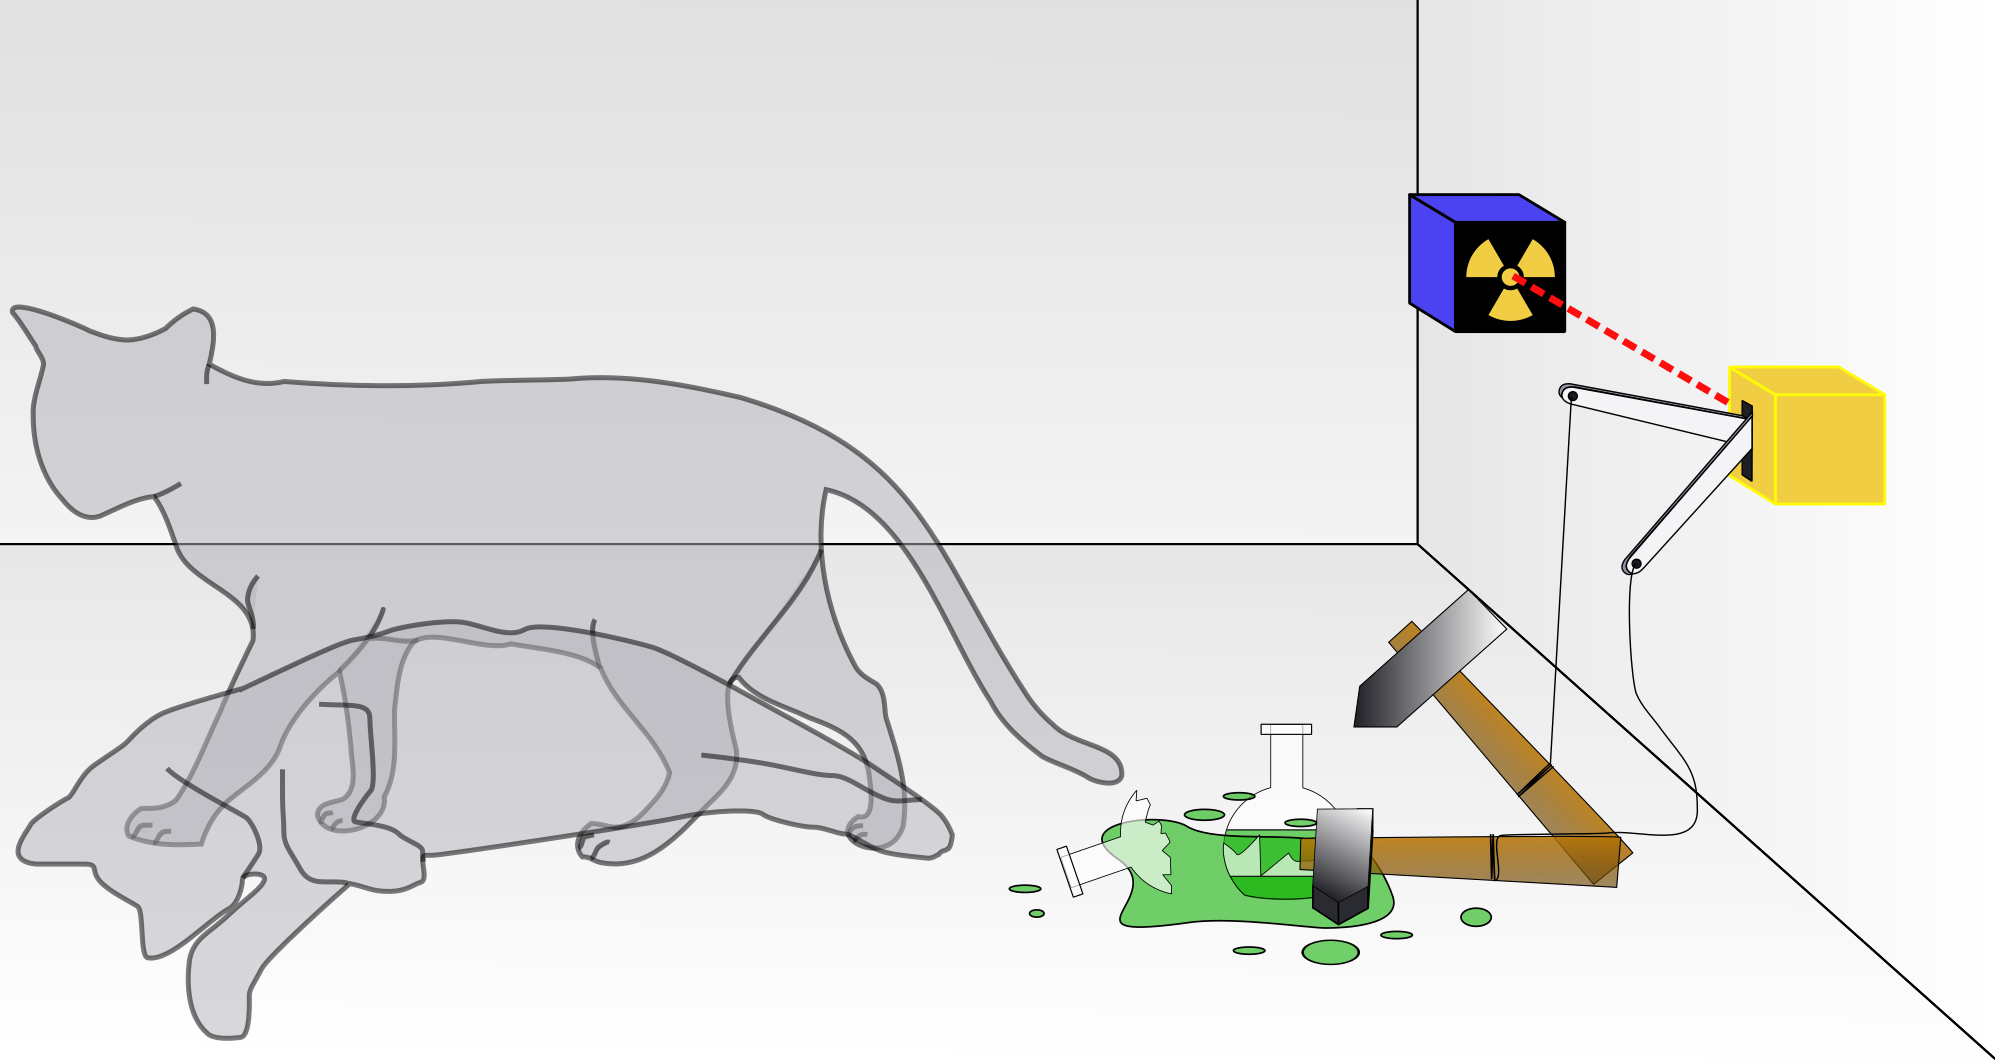
\includegraphics[width=100mm]{Chapter03/Schrodingers_cat.png}
  \caption[Caption for LOF]{A depiction of Schr\"{o}dinger's cat being both dead and alive.\protect\footnotemark}
  \label{deadlivecat}
  \end{figure}
  \footnotetext{ Original by Dhatfield. This image is licensed under the Creative Commons Attribution-Share Alike 3.0 Unported license. Source: https://commons.wikimedia.org/wiki/File:Schrodingers\_cat.svg}
  Such a distribution arises in this context because initially there is an atom that is in a superposition of decayed and non-decayed states, and so the expectation of $\hat{T}^{\mu\nu}(y)$ will have non-zero components both in the location where the non-decayed atom would be and also in the locations of the decayed atom and the particle the atom emitted. As the decayed atom part of the state interacts with the poison releasing device, this device will also enter into a superposition so that in both the location of the poison reservoir and in the locations of all the poison atoms in the container containing the cat and into which the poison is released, the expectation of $\hat{T}^{\mu\nu}(y)$ will have non-zero components. And then the cat will enter into a superposition of being in a dead state and an alive state, and so that the expectation of $\hat{T}^{\mu\nu}(y)$ will have non-zero components in locations where the dead cat ends up and where the living cat happens to be. So the expectation of $\hat{T}^{\mu\nu}(y)$ in the locations of the container containing the cat will be very different from what someone would actually observe.


